\section{Prototype}
In order to get a better idea of how the website should look like, various prototypes were drawn.
As they are prototypes, they are by no means a representation of the final product, but more of a source of inspiration and brainstorming, to consider when developing the website.
Throughout this section, one prototype sketch for each part of the website considered with prototyping, is presented, explained and discussed.

\begin{figure}[h]
	\centering
	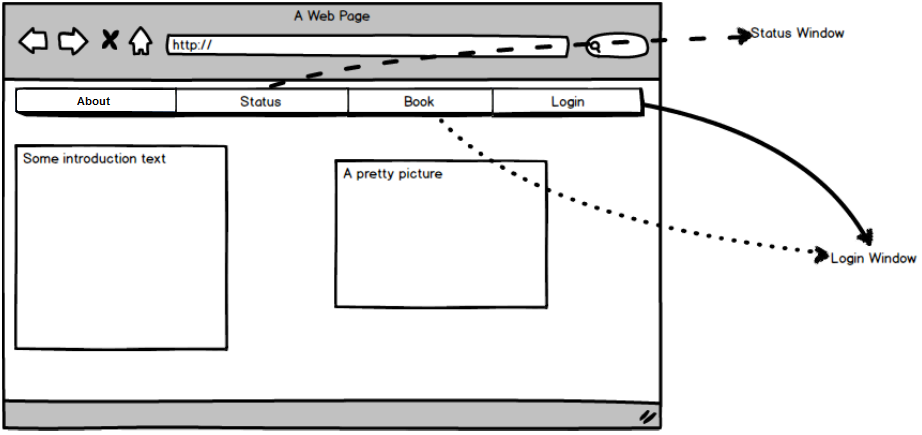
\includegraphics[scale=0.6]{design/prototype-about}
	\caption{About page.}\label{fig:prototype-about}
\end{figure}

First, we take a look at \figref{fig:prototype-about}.
This illustration presents a draft of the about page, it is structured as a standard about page with some description of the organisation behind the website as well as a pretty picture to look at.
What is more interesting to see in this illustration is the first draft of the menu bar.
The menu bar consists of links to about, status, book, and login links, each of which has their page(s) illustrated hereafter.


\begin{figure}[h]
	\centering
	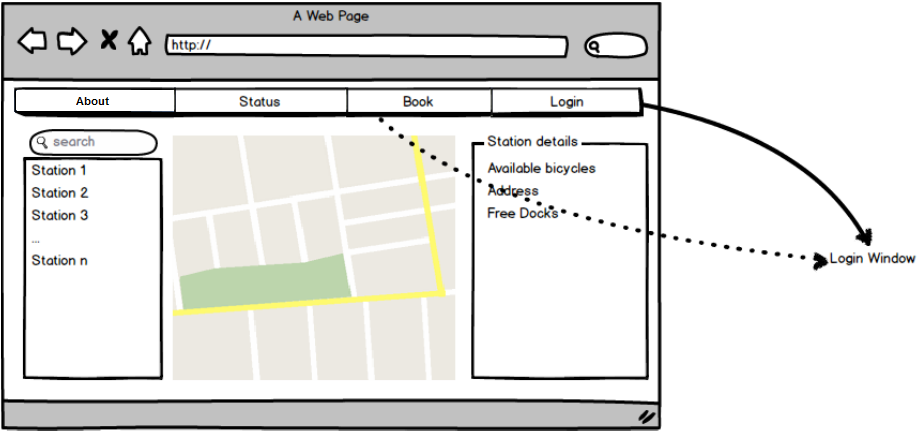
\includegraphics[scale=0.6]{design/prototype-status}
	\caption{Status page.}\label{fig:prototype-status}
\end{figure}

\begin{figure}[h]
	\centering
	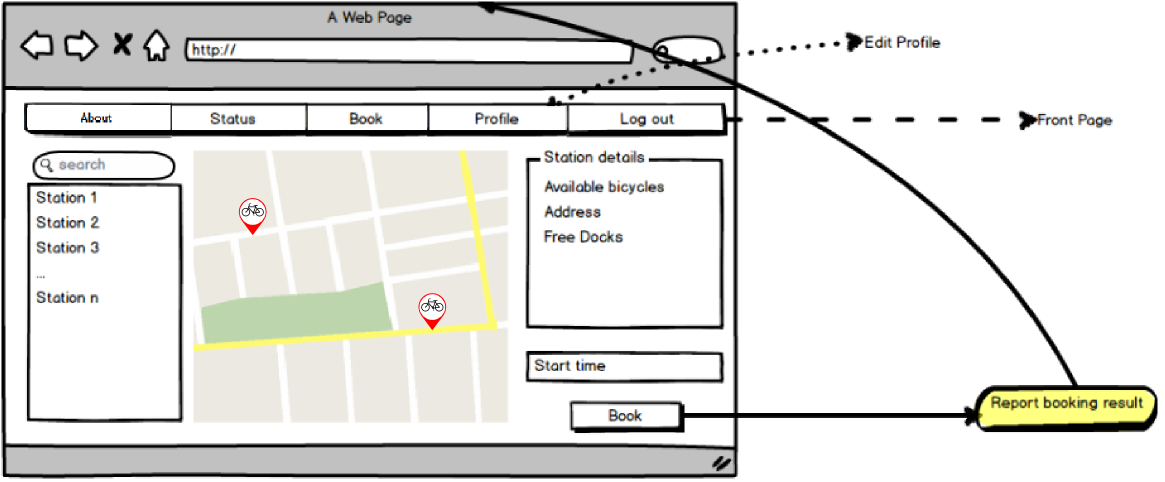
\includegraphics[scale=0.6]{design/prototype-booking}
	\caption{Booking page.}\label{fig:prototype-book}
\end{figure}

\begin{figure}[h]
	\centering
	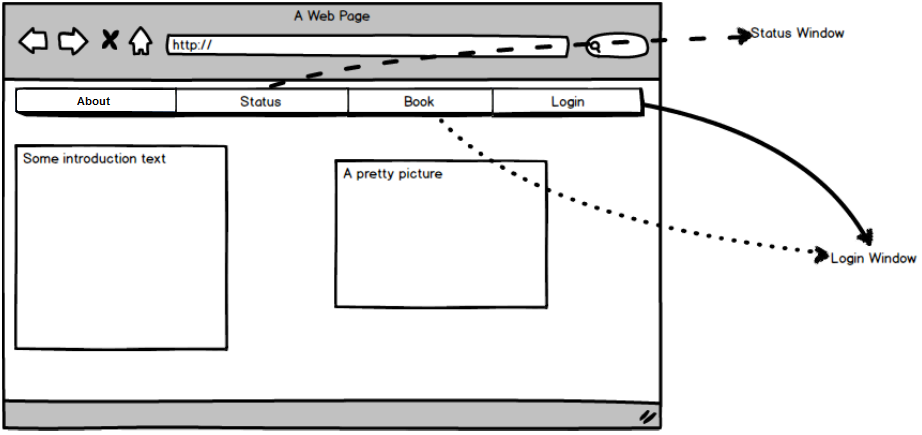
\includegraphics[scale=0.6]{design/prototype-about}
	\caption{Booking history page.}\label{fig:prototype-book-history}
\end{figure}

\begin{figure}[h]
	\centering
	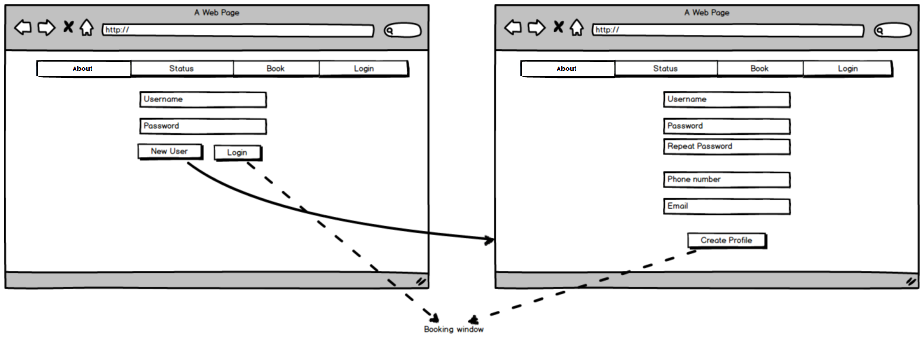
\includegraphics[scale=0.6]{design/prototype-user}
	\caption{User pages.}\label{fig:prototype-user-overall}
\end{figure}

\begin{figure}[h]
	\centering
	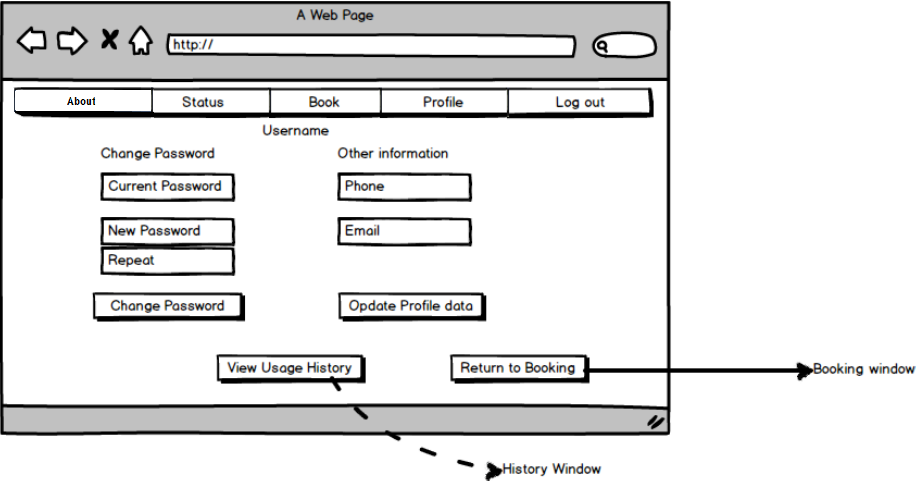
\includegraphics[scale=0.6]{design/prototype-edit-user}
	\caption{Edit user page.}\label{fig:prototype-edit-user}
\end{figure}
